\documentclass{standalone}

\usepackage{tikz}
\usetikzlibrary{positioning, fit,  shapes.geometric}
\usepackage{ifthen}
\usepackage{etoolbox}

\tikzset{
	backgroundcolor/.style ={fill=white},
	every node/.append style={
		minimum height=7mm,
	},
	labe/.append style={
		%Blue,
		align = center,
		backgroundcolor,
		fill opacity=0.6,
		text opacity=1,
		font={\footnotesize\itshape}	
	},
	layer/.append style={
		draw,
		align = center,
		minimum height=7mm,
	},
	tight/.append style={
		inner sep=0.2mm,
	},
	lookupbox/.append style={
		draw=none,
		append after command={
		       	[shorten <= -0.5\pgflinewidth]
		       	([shift={(-1.5\pgflinewidth,-0.5\pgflinewidth)}]\tikzlastnode.north east)
		       	edge([shift={( 0.5\pgflinewidth,-0.5\pgflinewidth)}]\tikzlastnode.north west) 
		       	([shift={( 0.5\pgflinewidth,-0.5\pgflinewidth)}]\tikzlastnode.north west)
		       	edge([shift={( 0.5\pgflinewidth,-1.5\pgflinewidth)}]\tikzlastnode.south west)            
		       	([shift={( -1.5\pgflinewidth,+0.5\pgflinewidth)}]\tikzlastnode.south east)
		       	edge([shift={(-1.5\pgflinewidth,-0.5\pgflinewidth)}]\tikzlastnode.north east)
		},
		inner sep=0.7mm,
		outer sep=0mm,
		minimum width=25mm
	}
}
\usetikzlibrary{calc}
\begin{document}

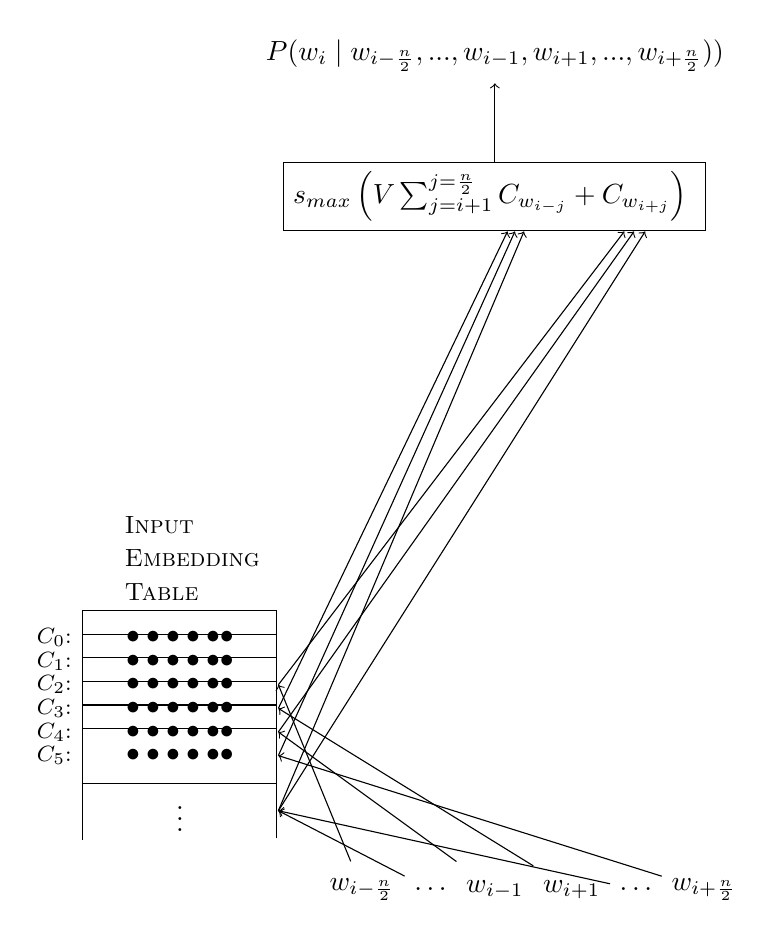
\begin{tikzpicture}[]


\node(wn1) at (0,0) {$w_{i-1}$};
\node(wp1) [right = 0mm  of wn1] {$w_{i+1}$};
\node(wn2)[left = 0mm of wn1] {$\ldots$};
\node(wp2)[right = 0mm of wp1] {$\ldots$};
\node(wn3)[left = 0mm of wn2] {$w_{i-\frac{n}{2}}$};
\node(wp3)[right = 0mm of wp2] {$w_{i+\frac{n}{2}}$};

\node(Cn)[lookupbox] at (-4,1) {$\vdots$};
\def\tblmax{6}
\foreach \ii in {1,...,\tblmax} {
	\pgfmathsetmacro\pos{(\ii - 1) * 3 };
	\pgfmathtruncatemacro\jj{(\tblmax -\ii)};
	
	\node(C\ii)[lookupbox, above = \pos mm of Cn]{$\bullet\bullet\bullet\bullet\bullet\bullet$};
	\node(Clbl\ii)[left = 0mm of C\ii]{\footnotesize $C_\jj$:};
};
\node(C)[above = 0mm of C\tblmax.north, text width=40] {\small \textsc{Input \\Embedding Table}};




\node(L2)[layer, above = 8 of wn1]{
$s_{max}\left(V \sum_{j=i+1}^{j=\frac{n}{2}} C_{w_{i-j}}+C_{w_{i+j}}\right)$
};


\path[->, draw] (wp1) to (C3.east) edge[->] (L2.290);
\draw[->] (wp2) to (Cn.east) edge[->] (L2.310);
\draw[->] (wp3) to (C1.east) edge[->] (L2.300);
\draw[->] (wn1) to (C2.east) edge[->] (L2.346);
\draw[->] (wn2) to (Cn.east) edge[->] (L2.347);
\draw[->] (wn3) to (C4.east) edge[->] (L2.345);




\node(out)[above = of L2]{$P(w_i \mid w_{i-\frac{n}{2}},..., w_{i-1}, w_{i+1},...,w_{i+\frac{n}{2}}))$};
\draw[->] (L2) edge (out);



\end{tikzpicture}

\end{document}